\documentclass[a4paper,12pt]{report}
\usepackage[utf8]{inputenc}
\usepackage[T1]{fontenc}
\usepackage[ngerman]{babel}
\usepackage[parfill]{parskip}
%\usepackage{eurosans}
\usepackage[top=3cm, left=3cm]{geometry}
\usepackage{setspace}
\usepackage{mdwlist}
\usepackage{graphicx}
\usepackage{eurosym}
\renewcommand*\familydefault{\sfdefault}

\setcounter{secnumdepth}{-1}

\begin{document}

\title{\textbf{Leitfaden für ESE-Tutoren 2015 für Masterstudenten}\\}
\date{}
\author{von\\Thomas Heinze, Berit Lochner, Denis Stein (2008), \\Marcus Hähnel und Nico Hoffmann (2009), \\Marius Melzer (2010), \\Robert Schädel (2011),\\Sascha Peukert (2013), \\Kilian Költzsch, Marc Satkowski und Sascha Peukert (2014), \\Philipp Heisig und Katja Linnemann (2015)}
\maketitle
\tableofcontents
\chapter{Hinweise für Tutoren}
\section{Ansprechpartner}
Katja (linnemann@ifsr.de): 01525/2879175\\
Philipp (heisig@ifsr.de): 0176/31101907 \\
FSR/ESE-Orga (ese-orga@ifsr.de): 0351/463-38226

\section{Aufgaben eines ESE-Tutors}
Als ESE-Tutor hast du die ehrenvolle Aufgabe, die Erstis an der Fakultät zu begrüßen und ihnen mit Tipps und Erfahrungen einen leichteren Einstieg ins Studium zu ermöglichen. Folgende Punkte solltest du beachten, damit das gelingt:
\begin{itemize}
	\item \textbf{Proud to be a Tutor:} Trage während der Woche zu allen ESE-Veranstaltungen (auch Abends) das ESE-Shirt und dein Namensschild.
	\item \textbf{Präsenz zeigen:} Sei während der ESE so oft wie möglich da, komme zum Frühstück usw. mit den Erstis ins Gespräch.
	\item \textbf{Have you met Ted:} Siehst du einen einsamen Ersti, hilf ihm, Anschluss zu finden (und hab Spaß dabei \Winkey ).
	\item \textbf{Sei hilfsbereit:} Ein Ersti fragt dich etwas oder ein Ersti guckt sich verloren um? Setze alles daran zu helfen!
\end{itemize}
\section{Anwesenheit in der ESE}
Eure Anwesenheit ist zu folgenden Zeiten ausdrücklich erforderlich:
\begin{itemize*}
	\item Aufgabenbereiche in denen ihr explizit als Helfer eingetragen seid
	\item Frühstück, Tütentragen und Begrüßung am Montag (ab 9 Uhr da sein)
	\item Einschreibung (Dienstag 8:30 Uhr, Treff vorm FRZ)
	\item Schnitzeljagd (Mittwoch 12:15 Uhr)
	\item ESE-Spiel (Donnerstag 12:15 Uhr)
\end{itemize*}
Während der Vorträge am Mittwoch und der Professorenvorstellung am Donnerstag müsst ihr natürlich nicht die ganze Zeit anwesend sein, an beiden Tagen könnt ihr in der Zeit auch gut Mittag essen gehen, damit ihr 12:15 pünktlich zur Vorbereitung der Schnitzeljagd/des ESE-Spiels da seid.\\
Die Anwesenheit zu allen anderen Veranstaltungen ist wünschenswert!

\section{Scheine}
Für die Teilnahme als Tutor an der ESE kann es einen Schein über 30h/1LP für die Allgemeine Basisqualifikation (Bachelor/Master) bzw. die Berufsspezifische Schlüsselkompetenz (Diplom) geben.\\
Bedingungen für die Vergabe eines Scheines:
\begin{itemize*}
	\item an Tutorenschulung teilgenommen (Ausschlusskriterium!)
	\item ein Tutorium geleitet (Ausnahmen nach Absprache möglich)
	\item Einschreibung, Schnitzeljagd und ESE-Spiel mit betreut
	\item min. eine weitere Aufgabe organisiert oder als Tutor betreut
	\item aktive Teilnahme an der Mehrheit der Veranstaltungen in der ESE-Woche
\end{itemize*}
Uns ist klar, dass es schwierig ist, allen Tutoren wirklich 30 Stunden Arbeit zuzuteilen -- trotzdem muss euer Einsatz erkennbar sein, damit wir euch einen Schein geben können. Sonst kann es ganz schnell passieren, dass wir in Zukunft keine Scheine mehr genehmigt bekommen...\\
Also: Wenn du einen Schein haben willst, sei zu allen wichtigen Veranstaltungen da und bring dich ein.

\section{Über das Tutorium}
Ziel des Tutoriums ist Vermittlung von Informationen rund um das Studium. Der Inhalt des zweiten Teils dieser Handreichung ist das Minimum, was ihr in den Tutorien vermitteln sollt, ihr könnt die Stichpunkte gerne noch mit eigenen Einfällen ergänzen.\\
Beachtet dabei:
\begin{itemize*}
	\item Die Informationen sollten möglichst \textbf{unparteiisch} und \textbf{nicht wertend} vermittelt werden.
	Insbesondere sollte man vermeiden, den Erstis schon vorab Angst vor bestimmten Vorlesungen oder Dozenten zu machen oder sie zum Nichtbesuchen der Vorlesungen zu animieren. Das betrifft auch das ESE-Spiel.
%	\item Eine Tutoriengruppe besteht aus zwei Tutoren und ca. 15-25 Erstis.
	\item Falls keiner der beiden Tutoren zu einem Thema eine Auskunft geben kann, verweist am besten auf erfahrenere ESE-Tutoren oder den FSR, anstatt (möglicherweise falsche) Spekulationen zu äußern. Montag Nachmittag wird das FSR-Büro besetzt sein, sodass ihr Leute mit spezifischeren Fragen auf Montag Nachmittag oder die Seminartutorien am Dienstag verweisen könnt.
%	\item Wie in den letzten Jahren hat jede Gruppe einen Namenspatron. Anhand dessen werden euch die Studenten nach der Begrüßung per Los zugeteilt.
\end{itemize*}

\section{Vor dem Tutorium zu erledigende Dinge}
\begin{itemize*}
\item Lest euch diesen Leitfaden schon mal im Ganzen durch. 
Es wäre schlecht, wenn ihr das erst im Tutorium selbst tun müsst! 
Markiert euch eventuell wichtige Punkte.
Wenn ihr Fragen habt, stellt diese beim Tutorentreffen oder per Mail.
\item Überlegt euch zusammen mit eurem Tutoriumspartner, wie ihr die Informationen vortragen wollt.
Möglicherweise wollt ihr bestimmte Dinge an die Tafel schreiben.
Vielleicht ist es am sinnvollsten, die Stichpunkte abwechselnd vorzutragen, damit der jeweils andere sich schon mal Gedanken zum nächsten machen kann.
\item Schaut in der unten stehenden Tabelle nach, wo euer Tutorium stattfindet. Den Raum bitte vorher schon mal suchen, falls ihr nicht sicher wisst, wo er sich befindet.
\item Am ESE-Montag bitte spätestens um 9:00 da sein und mit helfen (10:00 geht die Begrüßung mit den anschließenden Tutorien los)!
Wir treffen uns in der APB/E023 zum Frühstück.	
\end{itemize*}

\begin{center}
\vspace{1cm}
\begin{tabular}[h]{|l|l|l|l|}
	\hline
	\textbf{`'Namenspatron''} & \textbf{Tutor(en)} & \textbf{Raum}\\ \hline
	Master (alle) & Sebastian M. \&  Simon  \& Lars & INF/E023\\
	\hline
\end{tabular}
\end{center}

\chapter{Zu vermittelnde Informationen}

\section{Einführung}
\begin{itemize*}
\item Wenn ihr ausländische Studierende in eurer Gruppe habt, schickt sie bitte in den APB 1004 (Ratsaal). Das Tutorium ist von 11:10 – 13:30\\
\item Macht eine kleine Vorstellungsrunde, um euch kennenzulernen und die Atmosphäre ein bisschen aufzulockern. Auch wenn viele der Master-Erstis ihren Bachelor in Dresden gemacht haben, ist es dennoch wichtig für die zugezogenen Erstis.
Die Tutoren beginnen.
Am besten ihr erzählt, wie ihr heißt, wo ihr ursprünglich herkommt, was euch an der (Medien-) Informatik gefällt. 
Die Studenten könnten zusätzlich noch erwähnen, was sie vorher gemacht haben und wieso sie sich für das Inf/MInf-Studium in Dresden entschieden haben.
Schreibt am besten an die Tafel, was ihr gerne von den Erstis wissen möchtet.
\item Falls ihr eurer Gruppe anbieten wollt, auch nach dem Tutorium eventuell aufkommende Fragen zu beantworten, schreibt eure Emailadressen an die Tafel.
\end{itemize*}

\section{ESE-Woche}
\begin{itemize*}
\item ESE-Website: http://ese.ifsr.de (mit aktuellem Ablaufplan der ESE-Woche (da er sich auch in der Woche noch verändern kann), Weblinks, etc.)
\item Den Zeitplan gibt es auch im iCal Format (ICS Datei) auf ese.ifsr.de zum Download.
Kann man sich direkt in den Kalender importieren.
\item Der Ablaufplan der ESE wird am FSR-Büro hinter der Wendeltreppe hängen und auf der ESE-Webseite stehen.
\item Die wichtigen Dinge der ESE-Tüte durchgehen: NoPanic, Stundenplanauswahl (betrifft Master nicht), etc.
\item Geht die ESE-Woche durch und sagt kurz etwas zu den wichtigsten Programmpunkten für Master
\end{itemize*}
\vspace{0.5cm}
Ort der Begrüßung ist der Hörsaal POT/81 (Pothoff-Bau) und der der Vorträge ist die ganze Woche über die APB/E023.

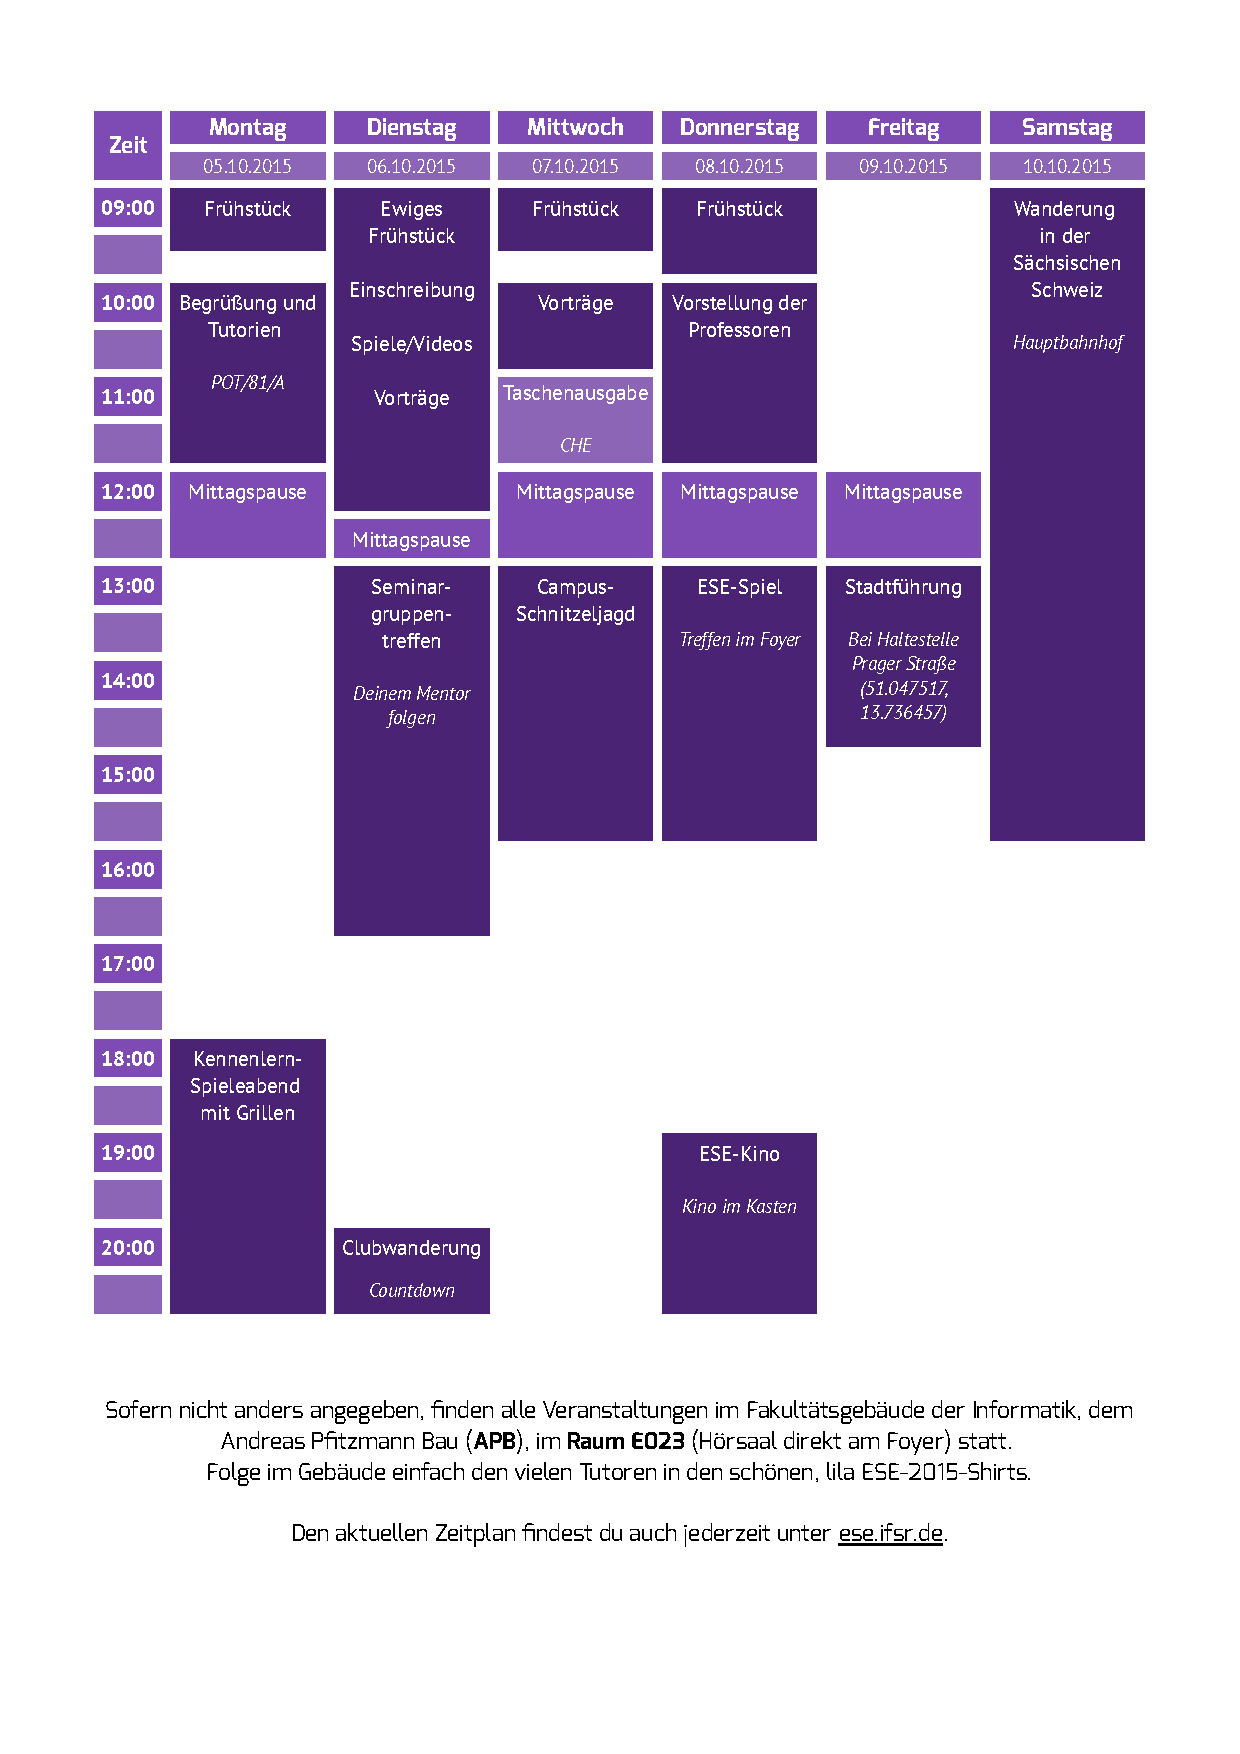
\includegraphics[width=\linewidth]{./zeitplan_2015.pdf}

\subsection{Montag}
\begin{itemize*}
\item 09:00 - 09:45 Frühstück
\item 10:00 - 11:00 Begrüßung im POT/0081
\item 11:00 - 12:00 Tutorien (siehe Tabelle auf S.2)
\item ab 12:00 Mittagspause
  \small{\textit{
  \begin{itemize*}
    \item Es wäre nett den Erstis einen gemeinsamen Mensabesuch anzubieten
    \item Mensakarten gibt es immer beim Frühstück oder nachher im FSR-Büro
    \item E-Meal aufladen erklären! Automaten, Infopoint, an der Kasse (Zeitersparnis)
    \item Am Nachmittag Sprechstunde im FSR-Büro
  \end{itemize*}
  }}
\item ab 18:00 Kennlern-Spieleabend mit Grillen (Fakultät Informatik)
\end{itemize*}

\subsection{Dienstag}
\begin{itemize*}
\item 09:00 - 12:30 Frühstück mit Entertainment, Vorträge, parallel Einschreibung
  \small{\textit{
  \begin{itemize*}
    \item Wichtig! Siehe nachfolgender Text zur Einschreibung
    \item Die Vorträge sind zu Studentischer Mitbestimmung und Auslandsstudium und werden als Block jeweils 2x angeboten (9:30 und 10:30)
  \end{itemize*}
  }}
\item 12:30 - 13:00 Mittagspause
\item ab 13:00 Erstes Seminargruppentreffen
  \small{\textit{
  \begin{itemize*}
    \item Wichtig! siehe nachfolgender Text zu Seminargruppen
    \item jeweils 13:00 und 15:00 je nach Studenplan/Seminargruppe
  \end{itemize*}
  }}
\item ab 20:00 Clubwanderung (Startet beim Studentenclub CountDown (Güntzstraße 22))
\end{itemize*}


\subsection{Mittwoch}
\begin{itemize*}
\item 09:00 - 09:45 Frühstück
\item 10:00 - 10:45 Vortrag Studienangelegenheiten und Organisation sowie TUDIAS
\item ab 11:00 Taschenausgabe der Uni am Chemiebau
\begin{itemize*}
  \item \small{\textit{die Vorträge enden so, dass die Erstis genug Zeit haben die Taschen zu ergattern}}
\end{itemize*}
\item 12:00 - 13:00 Mittagspause
\item 13:00 - 16:00 Campus-Schnitzeljagd
\begin{itemize*}
  \item \small{\textit{Tutorentreff Schnitzeljagd um 12:15 Uhr}}
\end{itemize*}
\end{itemize*}

\subsection{Donnerstag}
\begin{itemize*}
\item 09:00 - 10:00 Frühstück
\item 10:00 - 12:00 Vorstellung der Professoren
\item 12:00 - 13:00 Mittagspause
\item 13:00 - 16:00 ESE-Spiel
\begin{itemize*}
  \item \small{\textit{Tutorentreff ESE-Spiel um 12:15 Uhr}}
\end{itemize*}
\item ab 19:00 ESE-Kino im KIK (Kino im Kasten)
\end{itemize*}

\subsection{Freitag}
\begin{itemize*}
\item 13:00 - 15:00 Stadtführung
\begin{itemize*}
  \item \small{\textit{bitte erfragt grob das Interesse und gebt es weiter an Franz <franz@ifsr.de>}}
\end{itemize*}
\end{itemize*}

\subsection{Samstag}
\begin{itemize*}
\item 09:00 - ca. 16:00 Wanderung in der sächsischen Schweiz
\begin{itemize*}
  \item \small{\textit{bitte erfragt grob das Interesse und gebt es weiter an Lars <lars@ifsr.de>}}
\end{itemize*}
\end{itemize*}

\subsection{Einschreibung}
\begin{itemize*}
	\item Einschreibung zu Veranstaltungen variiert je nach Veranstaltung. Es wird jExam, Opal oder nichts genutzt.
	
	\item Optionale (aber ratsame!) Mailinglisten:
		\begin{itemize*}
		\item FSR-info ist der Verteiler des FSR über den regelmäßig Informationen zu den Vorgängen an der Fakultät und den Sitzungen des FSR kommen.
		\item extern: Jobangebote werden über diese Mailingliste verbreitet.
		\item und diverse andere,Einschreibung unter \\ https://www.ifsr.de/fsr:news:quicklinks\_fuer\_die\_einschreibung  (An die Tafel schreiben)
	\end{itemize*}
\end{itemize*}

\section{Studium}
\subsection{Allgemein}
\begin{itemize*}
	\item Alle wichtigen Infos: Prüfungs- und Studienordnung sowie Studienablaufplan und Modulbeschreibungen findet ihr auf der ESE-Webseite unter Infos
	\item Das wissen um Module und Lehrveranstaltungsformen wird vorausgesetzt.
	\item Prüfungen können zwei mal wiederholt werden
		\begin{itemize*}
			\item 1. Wiederholung: ein Jahr(zwei Semester) Zeit
			\item 2. Wiederholung: nochmals ein Semester Zeit
		\end{itemize*}
		2. Wiederholungsprüfung nicht geschafft $\rightarrow$ Exmatrikulation, Studium nicht geschafft
	\item wieder abmelden von einer Prüfung: ohne Angabe von Gründen bis 3 Werktage (bzw. 2 Wochen bei mündl. Prüfungen) vor dem Prüfungstermin möglich
	\item nach Ende dieser Frist: Rücktritt - nur bei Krankheit o.ä. zulässig\\ 
		muss Prüfungsamt unverzüglich schriftlich mitgeteilt werden (ärztliches Attest o.ä.)
	\item Prüfungsausschuss (je Studiengang): bearbeitet Anträge für Anerkennung bzw. Anrechnung von Studien- und Prüfungsleistungen, Anträge auf Prüfungsfristverlängerung, Anträge auf Annullierung einer Prüfung, etc.
	\item Regelstudienzeit überziehen: bis zu 4 Semester, danach Abschlussprüfung das erste Mal nicht bestanden, noch 1 Jahr Zeit für Wiederholung
	\item Studienzeit kann durch Uraubs- und Gremiensemester verlängert werden:
		\begin{itemize*}
			\item Urlaubssemester: studienfreies Semester, in dem neuerdings auch Prüfungen geschrieben werden können (valider Grund für Urlaubssemester nötig!)
			\item Gremiensemester: max. 3, Reduzierung der Fachsemesterzahl, kann man durch engagierte Gremienarbeit (Fachschaftsrat, Fakultätsrat, Prüfungsausschuss, etc.) bekommen
		\end{itemize*}	
\end{itemize*}
Eine Zusammenstellung von fürs Studium wichtigen Dokumenten und Links zu vielen Skripten findet man auch auf der FSR-Seite (ifsr.de $\rightarrow$ Studium).

\subsection{Master Informatik}
\begin{itemize*}
	\item \textbf{Basismodule:} 3 von 8 sind aus folgender Liste zu wählen zu wählen
	\begin{itemize*}
		\item Angewandte Informatik 	
		\item Künstliche Intelligenz 	
		\item Software- und Web-Engineering  
		\item Systemarchitektur 	
		\item Technische Informatik 	 
		\item Theoretische Informatik 
		\item Grafische Datenverarbeitung 
		\item Anwendungsfach
	\end{itemize*}	
	\item Das Anwendungsfach entspricht einem `'kleinen'' Nebenfach
	\item Auf http://web.inf.tu-dresden.de/Fak/w/15/stundenplan.html lassen sich alle Veranstaltungen des Semesters finden (meist mit Link zur jeweiligen Veranstaltungsseite).
	\item Bei den meisten Basismodulen muss man mindestens 2 Vorlesungen und 2 Übungen belegen und die restlichen 4 SWS sind frei wählbar. Trotzdem lieber in die Modulbeschreibung schauen!
	\item die gewählten Veranstaltungen in einem Basismodul werden zusammen in einer mündlichen Komplexprüfung geprüft.
	\item \textbf{Vertiefungsmodul:} Eines der Basismodule (nicht das Anwendungsfach) muss weiter vertieft werden. Der Ablauf ist analog, diesmal müssen aber 10 SWS belegt werden.
	\item \textbf{Profilmodule:} Die Veranstaltungen für die Profilmodule werden ebenfalls aus dem Katalog gewählt. Hierbei ist zu beachten dass die Module aufeinander aufbauen müssen. Wählt man eine Veranstaltung aus dem Grundlagenforschungsmodul, muss als nächstes eine Veranstaltung aus dem Katalog Forschungsprojekt Grundlagen gewählt werden. Wählt man eine Veranstaltung aus dem Anwendungsforschungsmodul, muss man als nächstes eine Veranstaltung aus dem Katalog Forschungsprojekt Anwendung wählen. In den meisten fällen umfasst das erste Modul eine Vorlesung mit Übung und das zweite Modul 1-2 Komplexpraktika. Nur das zweite Modul ist benotet.
	\item \textbf{Vertieftes Master-Praktikum:} Funktioniert analog zum 2.Profilmodul. Hier sind 8 SWS Komplexpraktika zu wählen.
	\item \textbf{Allgemeine Qualifikation:} Für dieses Modul sind Lehrveranstaltungen im Umfang von 180h zu erbringen. Dabei werden:  Sprachkurse und Vorlesungen mit 60h je 2SWS und Seminare / Workshops mit 30h je 2SWS angerechnet. 150h sind mit Angeboten anderer Fachbereiche/Fakultäten oder ausgewählten, benoteten Veranstaltungen der Fakultät Informatik (Tabelle 1) zu belegen. Dazu zählen:
	\begin{itemize*}
    		\item benotete Sprachkurse Englisch EBW F1, F2, F3 (Tudias)
    		\item benotete Sprachkurse (Tudias)
                     \item fachfremde, \textbf{benotete} Veranstaltungen im Bereich Studium Generale
	\end{itemize*}
	\item Die letzten 30h sind aus dem Angebot der Fakultät zu wählen (Hauptseminare). 
\end{itemize*}

\subsection{Master Medieninformatik}
\begin{itemize*}
	\item \textbf{Vertiefungsmodule:} 5 bzw. 6 von 10 sind aus folgender Liste zu wählen zu wählen
	\begin{itemize*}
		\item Software Engineering Ubiquitärer Systeme
		\item Multimedia Information Retrieval and Management
		\item Advanced Web-Engineering
		\item Advanced Multimedia User Interfaces
		\item Interaktionsdesign Theorie
		\item Interaktionsdesign Praxis
		\item Interaktionstechnologie für die künstlerische Praxis
		\item Basismodul Graphische Datenverarbeitung
		\item Angewandte Graphische Datenverarbeitung
		\item eLearning
		\item Multimodale Benutzungsoberflächen
	\end{itemize*}
	\item Je nach Modul müssen Veranstaltungen belegt werden, wie im Modulkatalog angegeben
	\item Es müssen Module von insgesamt 60 LP gewählt werden, die meisten Module haben 12 LP, manche aber auch nur 6 LP
	\item Lehrveranstaltungen können oftmals in mehrere Module eingebracht werden, daher ist zu empfehlen sich vor deren Prüfung eine grundlegende Studiums-Struktur zu überlegen
	\item \textbf{Brückenmodule:} 1 von 5 sind aus folgender Liste zu wählen
	\begin{itemize*}
		\item Verteilte Systeme und Internetdienste
		\item Data Management and Analytics
		\item Datenschutz und Datensicherheit
		\item Softwarearchitektur
		\item Softwareentwicklungs-Methoden
	\end{itemize*}
	\item Prinzipiell vom Umfang und Inhalt her ein weiteres Vertiefungsmodul mit anderem Themenkatalog
	\item \textbf{Ergänzungsmodule} 2 von 4  aus folgender Liste, oder das Anwendungsfach
	\begin{itemize*}
		\item Technisch-naturwissenschaftlicher Forschungs- und Anwendungskontext der Medieninformatik
		\item Geistes- und humanwissenschaftlicher Forschungs- und Anwendungskontext der Medieninformatik
		\item Kerngebiete der Informatik
		\item Master-Praktikum Medieninformatik
		\item Anwendungsfach
	\end{itemize*}
	\item Es ist zu empfehlen, das Anwendungsfach zu belegen, da (ausgenommen das Master-Praktikum) in den anderen Modulen oftmals nur wenige, bis gar keine Lehrveranstaltungen angeboten werden
	\item \textbf{Allgemeine Qualifikation:} Wie beim Master Informatik, es müssen 180h insgesamt belegt werden, davon 150h aus dem ersten Katalogteil mit verschiedenen Veranstaltungen wie Sprachkursen etc. und 30h aus dem zweiten Katalogteil, welcher prinzipiell aus Semniaren an der Inf. Fakultät besteht
\end{itemize*}

\section{Drucken, Kopieren, Rechentechnik}
\begin{itemize*}
	\item Das Rechenzentrum beinhaltet Computer-Arbeitsplätze, Wlan-Arbeitsplätze (Monitore mit VGA-Eingang, an die man sein Notebook anschließen kann), ein paar Spezialräume mit Multimedia-Equipment und eine Technik-Ausleihe (z.B. für Kameras, Beamer, etc.).
	Die meisten PCs haben einen Dualboot mit Windows und Linux (Ubuntu).
	\item Die Einschreibung in (die meisten) Übungen und das Abrufen der Prüfungsergebnisse geschieht über das elektronische Einschreibesystem jExam.
	Man findet es unter http://jexam.de.
% TODO: Format der E-Mail Adressen ist jetzt wie?
	\item Jeder Student hat ein Emailpostfach beim ZIH mit der Adresse sNR@mail.zih.tu-dresden.de.
	Neben POP3 und IMAP kann man die Mails auch über das Webinterface unter https://mail.zih.tu-dresden.de abrufen.
	Es ist wichtig, das Postfach regelmäßig abzurufen oder sich die Emails an eine andere Adresse weiterzuleiten, weil unter der Adresse u.a. Informationen über Prüfungsanmeldung, Rückmeldung zum kommenden Semester etc. ankommen.
	\item \textbf{Wichtig!} Falls noch nicht geschehen: Passwort noch heute im IDM ändern, damit morgen die Einschreibung funktioniert: https://idm-service.tu-dresden.de -- ruhig als Hausaufgabe aufgeben.
	\item Es gibt zwei WLAN-Netze auf dem Universitätsgelände.
	Das einfacher einzurichtende, aber unsicherere VPN/Web und das auch an anderen Universitäten (auch international) verwendete Eduroam.
	VPN/Web ist ein offenes Netzwerk.
	Nach dem Verbinden muss man seine Login-Daten nach dem Aufrufen der ersten Website im Browser eingeben.
	Zum Verwenden von Eduroam sollte man die Anleitung auf der Website der TU Dresden lesen und sich falls notwendig das benötigte Zertifikat herunterladen.
	Unter Linux funktioniert es mittlerweile mit allen wichtigen Networkmanagern (Gnome Network Manager, KNetworkmanager, wicd, auf der Konsole per wpasupplicant..).
	Unter aktuellen Versionen von Windows und OS X reicht es sich mit dem ZIH Login anzumelden.
	\item Der ZIH-Login gilt sowohl fürs Rechenzentrum als auch für jExam, Email und WLAN.
	Username ist die \glqq sNr\grqq, die auf den Immatrikulationsbögen steht.
	Passwort für den Erstlogin steht dort ebenfalls, ist aber wie bereits erwähnt dringendst abzuändern, da jegliche Funktionalität sonst stark eingeschränkt ist.
	\item Drucken und Kopieren ist möglich im FSR-Büro (ab 2ct/Seite), über eine beim Stura zu erwerbende Kopierkarte an unterschiedlichen Standorten in der Uni (http://www.fritzsche-steinbach.de/Download/Flyer\_TU\_Dresden.pdf -- 3,7-5ct/Seite), in der SLUB (5-15ct/Seite) oder an den diversen Copyshops auf dem Unigelände.
\end{itemize*}

\section{Studentische Selbstverwaltung}
\subsection{Fachschaftsrat}
Der Fachschaftsrat ist die Vertretung der Studenten auf Fakultätsebene.
Er besteht derzeit aus 17 Mitgliedern und wird immer im Wintersemester für ein Jahr neu gewählt.
Der FSR ist Ansprechpartner bei Fragen und Problemen und veranstaltet die ESE, Professorenstammtische, die Spieleabende, die Lehrevaluationen und diverse Turniere.
Die FSR-Sitzungen sind jede Woche Montags um 18:30 im Großen Ratssaal INF/1004 in der ersten Etage.
Die Sitzungen sind öffentlich, Gäste sind herzlich willkommen und die Protokolle findet man auf dem FTP-Server (ftp://ftp.ifsr.de), genauso wie Klausuren vergangener Jahre oder (fürs Hauptstudium / Master) Komplexprüfungsprotokolle.
Der FSR hat sein Büro in der INF/E017 (hinter der Treppe, neben dem Cafe ASCII).
Auf der Website ifsr.de gibt es Informationen zum Studium und Neuigkeiten rund um die Fakultät.
Auch als Ersti kann man sich gerne für den nächsten FSR zur Wahl stellen. Als Tutor natürlich erst recht :)

\subsection{Studentenrat}
Der Studentenrat, kurz StuRa, ist die Vertretung der Studenten auf Uniebene.
Er versucht studentische Interessen gegenüber der Universitätsleitung durchzusetzen, er verteilt Gelder und bietet Beratung zu BAföG, Sozialem und bei Rechtsfragen/-problemen.
Die Mitglieder sind Entsandte aus den FSRen der einzelnen Fakultäten.
Auch die Sitzungen des StuRa sind öffentlich und finden zweiwöchentlich an Donnerstagen ab 19:30 Uhr statt.

\section{Studentisches Leben}
\subsection{Studentenclubs}
In Dresden gibt es 16 Studentenclubs, die von ehrenamtlich von Studenten geführt werden.
Eine Auflistung gibt es z.B. unter http://www.vdsc.de (Vereinigung Dresdner Studentenclubs).
Der Studentenclub, der zur Fakultät Informatik \textit{gehört}, ist das \glqq CountDown\grqq\ in der Nähe des Straßburger Platzes.
\subsection{Kino}
Das Kino im Kasten ist ein Studentenkino und befindet sich an der Philosphischen Fakultät in der August-Bebel-Straße.
Mehr Informationen und das Kinoprogramm gibts unter http://kino-im-kasten.de.
Das KiK hat seit kurzem wieder geöffnet und freut sich über Besucher.

\section{Die Universität}
\subsection{SLUB}
Bei der Sächsischen Landes- und Universitätsbibliothek kann man sich als Student kostenlos anmelden und Bücher ausleihen oder sich in die ruhigen Räumlichkeiten zum Lernen setzen.
Die meisten Informatikbücher befinden sich in der Lehrbuchsammlung im Haupthaus und im gegenüberliegenden \glqq DrePunct\grqq.
\subsection{Mensen}
In allen Mensen der TU Dresden (Alte Mensa, Reichenbachstraße, Siedepunkt, Zeltmensa ...) kann man mit der \glqq Emeal\grqq-Karte bezahlen, die sich per Barzahlung an den Kassen, im Voraus per Kontozahlung am Automaten aufladen lassen oder per Selbstaufladung vom Konto bei Bedarf.
Die Mensakarten werden während der ESE beim Frühstück für einen Pfand von 5 Euro ausgegeben;
Wer noch keinen hat, kann auch im FSR-Büro vorbeikommen.

\subsection{Unisport}
Im Universitätssportzentrum kann man aus einer großen Anzahl von Sportarten wählen.
Die Einschreibung findet auf der Website des USZ (http://tu-dresden.de/ die\_tu\_dresden/zentrale\_einrichtungen/usz/) am Dienstag, den 14.10.2014 je nach Sportart ab 17.00 oder später statt.

\subsection{Sprachkurse}
Insgesamt bis zu 10 SWS Sprachkurse kann man kostenlos beim Sprachenzentrum LSK belegen.
Man kann je nach Kurs Sprachzertifikate bekommen oder einfach mal eine neue, fremde Sprachen erlernen.
Für den Informatik-Master wird Englisch benötigt.
Website: http://lskonline.tu-dresden.de.

\subsection{Nebenjobs}
SHKs (Studentische Hilfskräfte) werden überall an der Uni gesucht.
Viele informatikbezogene werden in der Fakultät per Aushang beworben oder über Ausschreibungen auf der Informatik Fakultätsseite.

\section{Wohnen in Dresden}
\begin{itemize*}
	\item Wenn man in Dresden seinen Hauptwohnsitz anmeldet bekommt man ein \glqq Begrüßunggeld\grqq\ von 150 Euro, das man beim Studentenwerk beantragen kann.
	\item Zweitwohnungssteuer: in Dresden fällig seit 2006, 10\% der jährlichen Netto-Kaltmiete (aber nur wenn echte Zweitwohnung; http://www.dresden.de/media/ pdf/infoblaetter/Handzettel\_Info\_Zweitwohnungssteuer.pdf).
	Als Bewohner einer WG oder eines Wohnheimes kann man allerdings Widerspruch einlegen und muss die Steuer nicht zahlen.
	\item Den neuen Wohnsitz sollte man innerhalb von 14 Tagen bei den Meldestellen angeben (http://dresden.de/de/02/or/anliegen/c\_241.php).
	\item Im Studentenheim sind am Anfang des Semesters meist bereits keine Plätze mehr frei.
	Fragen kann man aber trotzdem.
\end{itemize*}

\section{Dresden}

\subsection{Altstadt}
\begin{itemize*}
	\item Kulturelles Zentrum: Semperoper, Zwinger, Frauenkirche,...
	\item Einkaufsmeile
\end{itemize*}

\subsection{Neustadt}
\begin{itemize*}
	\item Kneipenviertel
	\item viele Programmkinos: Schauburg, Casablanca, Thalia,...
	\item einmal im Jahr großes Straßenfest: BRN - Bunte Republik Neustadt.
\end{itemize*}

\section{Ansprechpartner bei Problemen}
\begin{itemize*}
	\item FSR: fsr@ifsr.de
	\item Studiendekan: Prof. Weber (allgemein), Prof. Friedrich (Lehramtsstudiengänge), Prof. Hölldobler (englischsprachige Studiengänge).
	\item Studentische Studienberatung: Sascha Peukert (studienberatung-inf@ifsr.de) und Kilian Költzsch (studienberatung-minf@ifsr.de) oder beide unter studienberatung@ifsr.de.
	\item studentische Vertreter im Prüfungsausschuss: Sascha Peukert, Duc Tien Nguyen.
	\item Prüfungsamt (INF/3039 und 3040).
	\item Rechtsverbindliche Auskünfte gibt es aber nur vom Prüfungsausschuss, Anträge über das Prüfungsamt stellen!
\end{itemize*}

\section{Rundgang durch die Fakultät}
Macht einen kleinen Rundgang durch die Fakultät und zeigt mindestens: ASCII, FSR-Büro, E023 (Vorlesungssaal), Rechenzentrum, Prüfungsamt.
Anschließend könnte man in die Alte Mensa mensen gehen.


\end{document}
